\documentclass[../main.tex]{subfiles}
\begin{document}
  \chapter{Lecture 2}
    \paragraph{Reminder}
    Material derivative 
    \begin{displaymath}
      \dfrac{}{t} = \frac{D}{Dt} = \ptf{}{t} + \vec u \cdot \nabla \cdot
    \end{displaymath}

    Mass conservation implies the continuity equation
    \begin{displaymath}
      \ptf{\rho}{t} + \nabla \cdot ( \rho \vec u ) = 0.
    \end{displaymath}

    \paragraph{New stuff}
    Expanding the above equation we obtain
    \begin{displaymath}
      \underbrace{\ptf{\rho}{t} + \vec u \cdot \nabla \rho}_{\dfrac{\rho}{t}} + \rho \nabla \cdot \vec u = 0,
    \end{displaymath}
    and thus
    \begin{displaymath}
      \frac{1}{\rho} \dfrac{\rho}{t} = - \nabla \cdot \vec u. 
    \end{displaymath}
    If we introduce \fndef{specific volume} $\nu = 1 / \rho$ we obtain
    \begin{displaymath}
      \frac{1}{\nu} \dfrac{\nu}{t} = \nabla \cdot \vec u.
    \end{displaymath}

    We introduced that because we want to study incompressible flow.
    If the flow is incompressible we express it by saying that
    \begin{displaymath}
      \dfrac{\rho}{t} = 0 \quad \tm{or}\quad  \dfrac{\nu}{t} = 0.
    \end{displaymath}
    From the continuity equation incompressibility of the flow implies that
    \begin{displaymath}
      \nabla \cdot \vec u = 0.
    \end{displaymath}
    
    For the incompressible flow the $\vec u$ is divergence-free or solonoidal (\todo I didn't hear well).

    If $\nabla \cdot \vec u = 0$ and $ f(\vec r, t) = f_0 = \tm{const}$ then\footnote{It follows from the continuity equation.}
    \begin{displaymath}
      \forall t \quad f(\vec r, t) = f_0 = \tm{const}.
    \end{displaymath}

    Positive divergence implies expansion, negative implies compression.
    

    \section{Newton's second law (Momentum balance)}
    % \fndef{Material volume}. 
    Consider a closed system (volume $V(t)$) which is comprised of the same fluid particles
    (it flows with a fluid). 

    % \todo Fig0.
    \begin{figure}[h]
      \centering
      \begin{tikzpicture}
        \node[anchor=south west] (image) at (0,0)
        {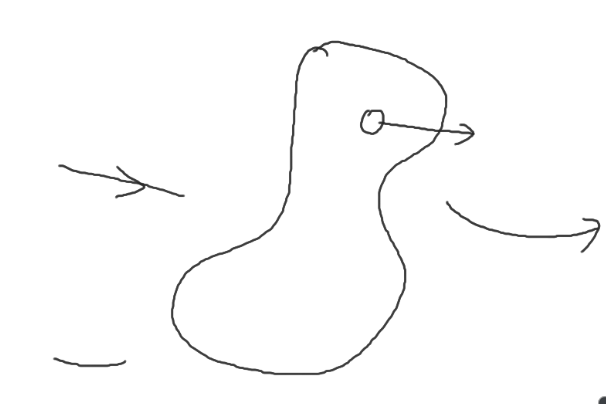
\includegraphics[width=0.25\textwidth]{./images/01Fig0.png}};
          \begin{scope}[x={(image.south east)}, y={(image.north west)}]
          \node at (0.0, 0.0) {};
          \end{scope}
      \end{tikzpicture}
      % \caption{}
    \end{figure}

    We want to calculate the momentum of such \fndef{material volume}.
    It is obviously an integral
    \begin{displaymath}
      \vec P (t) = \int_{V(t)} \rho(\vec r, t) \vec u(\vec r, t) \d \vec r.
    \end{displaymath}
    That is a linear momentum of the material volume.
    We want to state the Newton second law:
    \begin{displaymath}
      \dfrac{\vec P(t)}{t} = \vec F, 
    \end{displaymath}
    where $\vec F$ is the net force.
    \begin{displaymath}
      \dfrac{\vec P}{t} = \dfrac{}{t} \int_{V(t)} \rho(\vec r, t) \vec u (\vec r, t) \d \vec r = ?.
    \end{displaymath}
    
    Here is a theorem (i.e. fancy name for Leibniz rule):
    
    \begin{theorem}[Raynold's transport theorem]
      \begin{displaymath}
        \dfrac{}{t} \int_{V(t)} \beta (\vec r, t) \d \vec r = 
        \int_{V}\left[ \ptf{\beta}{t} + \nabla \cdot (\beta \vec u) \right] \d \vec r
        = \int_V \left[ \ptf{\beta}{t} + \vec u \cdot \nabla \beta + \beta \nabla \cdot \vec u \right]
        ,
      \end{displaymath}
      where $V$ is a fixed quantity, called control volume (i.e. any volume that coincides with $V(t)$).
    \end{theorem}

    The things that contribute to this change can be interpreted as
    \begin{enumerate}
      \item local change $\ptf{\beta}{t}$,
      \item advection i.e. $\vec u \cdot \nabla \beta$,
      \item changing volume i.e. $\beta \nabla\cdot \vec u$.
    \end{enumerate}

    Applying RTT to the momentum we get
    \begin{displaymath}
      \dfrac{\vec P }{t} = \dfrac{}{t} \int_{V(t)} \rho \vec u \d \vec r 
      = \int_V \left[ \ptf{\rho\vec u }{t} + \nabla \cdot (\rho \underbrace{\vec u \vec u}_{\vec u \otimes \vec u}) \right]
    \end{displaymath}
    
    \paragraph{Homework} Show that if $\beta = \rho b$, then 
    \begin{displaymath}
      \dfrac{}{t} \int_{V(t)} \rho b \d \vec r = \int_{V} \rho \dfrac{b}{t} \d \vec r,
    \end{displaymath}
    using RTT (Raynold's transport theorem) and the continuity equation.
    
    \begin{displaymath}
      \frac{\xi }{ x} = \int_V \d V 
    \end{displaymath}
    
    \begin{displaymath}
      \dfrac{\vec P}{t} = \dfrac{}{t} \int_{V(t)} \rho \vec u \d \vec r 
      = \int_V \rho \dfrac{\vec u}{t} \d \vec r 
      = \vec F,
    \end{displaymath}
    and thus the integral's form of Newton second law
    \begin{displaymath}
      \int_V \rho \dfrac{\vec u}{t} \d \vec r = \vec F.
    \end{displaymath}
    
    \section{Further consequences of RTT}
    % \todo Fig1.

    \begin{figure}[ht]
      \centering
      \begin{tikzpicture}
        \node[anchor=south west] (image) at (0,0)
        {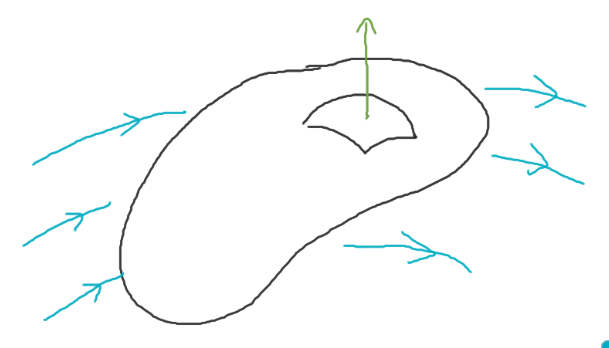
\includegraphics[width=0.25\textwidth]{./images/01Fig1.png}};
          \begin{scope}[x={(image.south east)}, y={(image.north west)}]
          \node at (0.0, 0.0) {};
          \end{scope}
      \end{tikzpicture}
    \end{figure}

    
    \begin{displaymath}
      M = \int_V \rho \d \vec r \qLRa \ptf{M}{t} 
      = \ptf{}{t} \int_V \rho \d \vec r 
      = \int_V \ptf{\rho}{t} \d \vec r 
      = - \int_V \nabla \cdot (\rho \vec u) \d \vec r
      = - \int_{\partial V} \rho \vec u \cdot \hat n \d S .
    \end{displaymath}

    To note: material volume is the volume that flows with the fluid.
    

    Consider a material volume $V(t)$ and its mass given by
    \begin{displaymath}
      M = \int_{V(t)}  \rho \d \vec r.
    \end{displaymath}
    The mass conservation means that
    \begin{displaymath}
      \dfrac{M}{t} = 0.
    \end{displaymath}

    We calculate
    \begin{displaymath}
      \dfrac{M}{t} = \dfrac{}{t} \int_{V(t)} \rho \d \vec r 
      = \int_V \left[ \ptf{\rho}{t} + \nabla \cdot (\rho \vec u) \right]\d \vec r 
      = 0.
    \end{displaymath}
    The above equation states that the mass of the material volume which travels with the flow remains constant.
    
    \paragraph{Force model}
    In the following equation
    \begin{displaymath}
      \int_V \rho \dfrac{\vec u}{t} \d \vec r = \vec F,
    \end{displaymath}
    we do not know what $\vec F$ is and therefore need a model for it.

    % \todo Fig3 TODO
    \begin{figure}[h]
      \centering
      \begin{tikzpicture}
        \node[anchor=south west] (image) at (0,0)
        {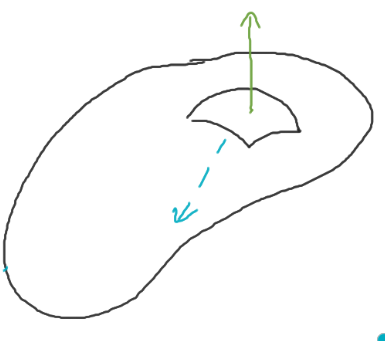
\includegraphics[width=0.25\textwidth]{./images/01Fig2.png}};
          \begin{scope}[x={(image.south east)}, y={(image.north west)}]
          \node at (0.0, 0.0) {};
          \end{scope}
      \end{tikzpicture}
    \end{figure}

    Consider that the fluid acts on its surface element $\d a$ (with a normal vector $\hat n$).
    Let $\vec t$ be a force per unit area, and $\d \vec F = \vec t \d a$.
    \begin{displaymath}
      \vec F \os{\tm{model}}{=} \int_{\partial V} \d \vec F 
      = \int_{\partial V}  \vec t \d a
      = - \int_V \nabla p \d \vec r.
    \end{displaymath}
    Assume that $\vec t = - p \hat{n}$, where $p $ is a pressure and $\nabla p $ a \fndef{pressure field}.
    
    \begin{displaymath}
      \int_V \rho \dfrac{\vec u }{t} \d \vec r = - \int_V \nabla p \d \vec r,
    \end{displaymath}
    \begin{displaymath}
      \int_V \left[ \rho \dfrac{\vec u}{t} + \nabla p \right]\d \vec r = 0 
      \qLRa \rho \dfrac{ \vec u }{t} = - \nabla p.
    \end{displaymath}
    We may also write it as 
    \begin{displaymath}
      \rho \left( \ptf{\vec u}{t} + \vec u \cdot \nabla \cdot \vec u  \right) = - \nabla p.
    \end{displaymath}
    This is the \fnvi{Euler model of the ideal fluid} (ideal fluid without dissipation).
    
    \section{Equilibrium}
    Equilibrium is obtained when $\vec u = 0$ and thus $\nabla p = 0$
    (especially if $p = \const$).
    \begin{itemize}
      \item ideal fluid $ \vec t = - p \hat n$
      \item In general $ \vec t = \ten{\Sigma}^T \cdot \vec n$, where $\Sigma$ is a \fndef{Cauchy stress tensor} (second order tensor).
    \end{itemize}
    In general case force can have a form 
    \begin{displaymath}
      \vec F = \int_{\partial V} \vec t \d a = \int_{\partial V} \ten{\Sigma}^T \cdot \hat n \d a 
      = \int_V \nabla \cdot \ten{\Sigma} \d \vec r,
    \end{displaymath}
    with the stress tensor
    \begin{displaymath}
      \ten{\Sigma} = - p \cdot\ten{1} + \ten{\Sigma}'. % TODO that's not all correct. 
    \end{displaymath}


    Newton's second law
    \begin{displaymath}
      \int_V \rho \dfrac{\vec u}{t} \d \vec r = \int\nabla \cdot \ten \Sigma \d \vec r.
    \end{displaymath}

    \begin{displaymath}
      \ten \Sigma = \underbrace{- p \ul{\ul{1}}}_{\tm{ideal term}} + \underbrace{\ul{\ul{\Sigma}}}_{\tm{deviatory part}}
    \end{displaymath}
    Deviatoric part vanishes in equilibrium.

    Ideal fluid model $\ten \Sigma' = 0$, $\ten \Sigma = - p \ul{\ul{1}}$.
    \begin{displaymath}
      \nabla \cdot \Sigma = \nabla \left( - p \ul{\ul{1}} \right) = - \nabla p.
    \end{displaymath}

    \paragraph{Summary}
    Til now we formulated
    
    \begin{itemize}
      \item Continuity equation
        \begin{displaymath}
            \ptf{\rho}{t} + \nabla \cdot ( \rho \vec u ) = 0
        \end{displaymath}
      \item Newton's law
        \begin{displaymath}
          \rho \left( \ptf{\vec u }{t} + \vec u \cdot \nabla \cdot \vec u  \right) = \nabla \cdot \ten \Sigma
      \end{displaymath}
    \item What's next? Angular momentum.
    \end{itemize}

    \section{Angular momentum}
    \begin{figure}[h]
      \centering
      \begin{tikzpicture}
        \node[anchor=south west] (image) at (0,0)
        {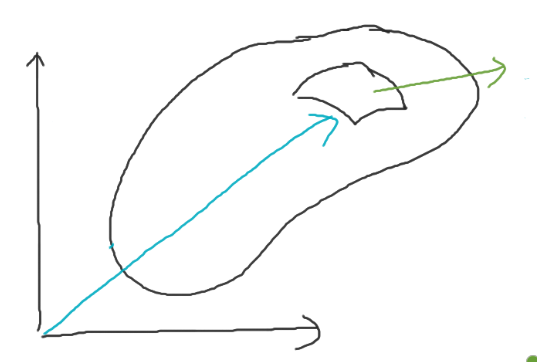
\includegraphics[width=0.25\textwidth]{./images/01Fig3.png}};
          \begin{scope}[x={(image.south east)}, y={(image.north west)}]
          \node at (0.0, 0.0) {};
          \end{scope}
      \end{tikzpicture}
    \end{figure}

    Consider a material volume $V(t)$, with density $\rho$ and a point at $\vec r$ moving with a velocity $\vec u$.
    \begin{displaymath}
      \vec L (t) = \int_{V(t)}\vec r \times \rho \vec u \d \vec r
      = \int_{V(t)} \rho (\vec r \times \vec u) \d \vec r
      = \int_{V(t)} \rho \vec l \d \vec r,
    \end{displaymath}
    where $\vec l = \vec r \times \vec u $ is the \fndef{angular momentum per unit mass}.

    The law of the change of the angular momentum
    \begin{displaymath}
      \dfrac{ \vec L }{t} = \vec N,
    \end{displaymath}
    where $\vec N$ is a net torque acting on $V(t)$.
    \begin{displaymath}
      \dfrac{\vec L}{t} = \dfrac{}{t} \int_{V(t)} \rho \vec l \d \vec r \os{\tm{RTT + cont}}{=\joinrel=} \int_V \rho \dfrac{\vec l}{t} \d \vec r.
    \end{displaymath}
    We calculate $\vec N$ by
    \begin{displaymath}
      \vec N = \int_{\partial V} \vec r \times\vec t \d a.
    \end{displaymath}

    \begin{displaymath}
      \int_V \rho \dfrac{\vec l}{t} \d \vec r = \int_{\partial V} \vec r \times \vec t \d a 
      = \int_{\partial V} (\vec r \times \Sigma^T) \cdot \hat n \d a 
    \end{displaymath}
    using divergence theorem
    \begin{equation}
      = \int_V \nabla \cdot \left[ ( \vec r \times \Sigma^T)^T \right] \d \vec r.
      \label{eq:prev}
    \end{equation}

    where the divergence theorem reads
    \begin{displaymath}
      \int_{\partial V} T \cdot \hat n \d a = \int_V \nabla \cdot T^T  \d \vec r.
    \end{displaymath}

    Going back to \ref{eq:prev}
    \begin{displaymath}
       = \int_V \left[ \vec r \times \nabla \cdot \Sigma - 2 \vec \sigma \right] \d \vec r,
    \end{displaymath}
    where $\vec \sigma $ is the axial vector associated with $\Sigma$.
    Thus
    \begin{displaymath}
      \int_V \rho \dfrac{ \vec l}{t} \d \vec r = \int_V \left[ \vec r \times \nabla \cdot \Sigma - 2 \vec \sigma \right] \d \vec r ,
    \end{displaymath}
    and since the volume $V$ can be anything we get
    \begin{equation}
      \rho \dfrac{ \vec l }{t} = \vec r \times \nabla \cdot \Sigma - 2 \vec \sigma.
      \label{eq:2.2}
    \end{equation}

    This is too complicated, we need to simplify it.
    
    \begin{displaymath}
      \rho \dfrac{ \vec l }{t} = \rho \dfrac{\vec r \times \vec u}{t} 
      = \rho \vec r \times \dfrac{\vec u}{t} + \rho \dfrac{ \vec r }{t} \times \vec u
      = \vec r \times \underbrace{\rho \dfrac{\vec u}{t}}_{\nabla \cdot \ten \Sigma} 
      = \vec r \times \nabla \cdot \ten \Sigma.
    \end{displaymath}

    Substituting it to  \ref{eq:2.2} we get
    \begin{displaymath}
      \vec \sigma = 0.
    \end{displaymath}
    Thus the $\Sigma $ is symmetric.

    The stress tensor need not to be symmetric for magnetic fluids (it works for simple fluids).


    \paragraph{,,Complex'' fluids}
    % \begin{figure}
    %   \centering
    %   \begin{tikzpicture}
    %     \node[anchor=south west] (image) at (0,0)
    %     {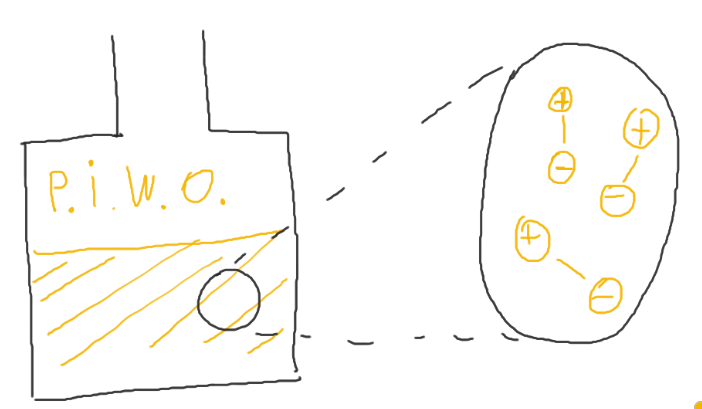
\includegraphics[width=0.25\textwidth]{./images/01Fig4.png}};
    %       \begin{scope}[x={(image.south east)}, y={(image.north west)}]
    %       \node at (0.0, 0.0) {};
    %       \end{scope}
    %   \end{tikzpicture}
    % \end{figure}

    Consider a magnetic fluid in a bottle, with magnetic dipoles.
    Assume that we apply a magnetic field, so there is a reorientation and an \fndef{internal torque} appears.
    
    \begin{displaymath}
      \vec N = \int_{\partial V} \vec r \times \vec t \d a + \int_{V} \vec b \d \vec r,
    \end{displaymath}
    where $\vec b$ is the internal torque.
    
    
    \section{Energy conservation}
    \begin{figure}
      \centering
      \begin{tikzpicture}
        \node[anchor=south west] (image) at (0,0)
        {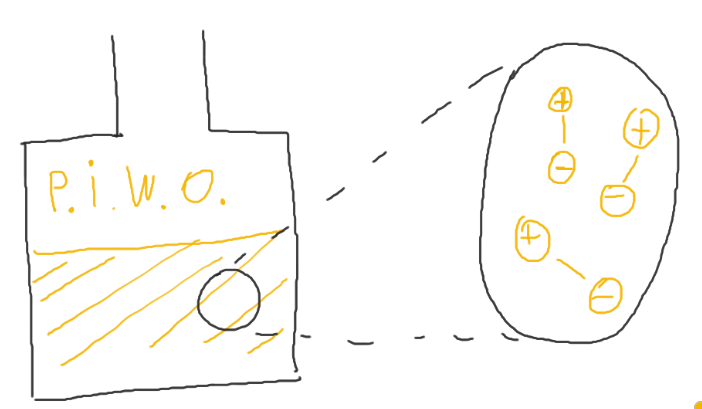
\includegraphics[width=0.25\textwidth]{./images/01Fig4.png}};
          \begin{scope}[x={(image.south east)}, y={(image.north west)}]
          \node at (0.0, 0.0) {};
          \end{scope}
      \end{tikzpicture}
    \end{figure}

    Consider a material volume $V$ and a small surface element $\d a$.
    The energy is given by 
    \begin{displaymath}
      E(t) = \int_{V (t)} \rho (\vec r ,t ) e (\vec r, t) \d \vec r ,
    \end{displaymath}
    where $e (\vec r, t)$ is the energy for unit mass.

    The ,,law'' of change
    \begin{displaymath}
      \dfrac{E}{t} = \dfrac{W}{t} + \dfrac{Q}{t},
    \end{displaymath}
    where $W$ is a mechanical work and $Q$ is a heat.

    Using RTT and continuity we get
    \begin{displaymath}
      \dfrac{E}{t} = \dfrac{}{t} \int_{V(t)} \rho e \d \vec r = \int_V \rho \dfrac{e}{t} \d \vec r,
    \end{displaymath}
    
    \begin{displaymath}
      \dfrac{W}{t} = \int_{\partial V } \vec t \cdot \vec u \d a 
      = \int_{\partial V} (\ten \Sigma^T \cdot \vec u ) \cdot \hat n  \d a 
      = \int_V \nabla \cdot ( \ten \Sigma \cdot u) \d \vec r.
    \end{displaymath}

    \begin{displaymath}
      \dfrac{Q}{t} = - \int_{\partial V} \vec q \cdot  \hat n \d a = - \int_V \nabla \cdot \vec q \d \vec r,
    \end{displaymath}
    where $\vec q$ is the heat flow per unit surface per unit time. % TODO upewnić się, że to jest rzeczywiście to 

    Summing up we get
    \begin{equation}
      \rho \dfrac{ e}{t} = \nabla \cdot ( \Sigma \cdot \vec u) - \nabla \cdot \vec q.
      \label{eq:2.3}
    \end{equation}

    Let's introduce the separation 
    \begin{displaymath}
      e = e_0 + \frac{1}{2} \vec u^2.
    \end{displaymath}

    Substituting it into \ref{eq:2.3} we obtain
    \begin{displaymath}
      \rho \dfrac{e_0}{t} = - \rho \dfrac{}{t} \left( \frac{1}{2} \vec u^2 \right) + \nabla \cdot (\Sigma \cdot \vec u ) - \nabla \cdot \vec q.
    \end{displaymath}
    \begin{displaymath}
      \rho \dfrac{}{t} \left( \frac{1}{2} \vec u ^2  \right) 
      = \vec u \cdot \rho \dfrac{\vec u}{t} 
      = \vec u \cdot ( \nabla \cdot \Sigma) 
      = \nabla \cdot ( \Sigma \cdot u) - \Sigma :\nabla \vec u % TODO Double contraction of tensors
    \end{displaymath}
    
    For the internal energy $e_0$:
    \begin{displaymath}
      \rho \dfrac{e_0}{t} = \Sigma : \nabla \vec u - \nabla \cdot \vec q.
    \end{displaymath}
    
    For $\Sigma = - p \ul{\ul{1}} + \Sigma'$
    \begin{displaymath}
      \Sigma : \nabla \vec u = - p ( \nabla \cdot \vec u) + \Sigma' : \nabla \vec u.
    \end{displaymath}
    
    \section{Ideal fluid approximation}

    We assume no deviatoric stress, and no heat flows
    \begin{align*}
      \Sigma' = 0 \\
      \vec q = 0.
    \end{align*}
    For the ideal fluid
    \begin{displaymath}
      \rho \dfrac{e_0}{t} = - p ( \nabla \cdot \vec u).
    \end{displaymath}

    This approximation is a result of assuming that the particles move all together, 
    so there is no viscosity and also no way to conduct a heat.
    
    For a compressible flow
    \begin{itemize}
      \item $\nabla \cdot \vec u > 0 \qLRa \dfrac{e_0}{t} < 0 $ (expansion),
      \item $\nabla \cdot \vec u < 0 \qLRa \dfrac{e_0}{t} > 0 $ (compression),
    \end{itemize}
    and for the incompressible flow there is no way to change internal energy, $\dfrac{e_0}{t} = 0$.
    In ideal fluid there is no dissipation.
    However the real fluids do.

    \section{Entropy balance} 
    \begin{figure}[h]
      \centering
      \begin{tikzpicture}
        \node[anchor=south west] (image) at (0,0)
        {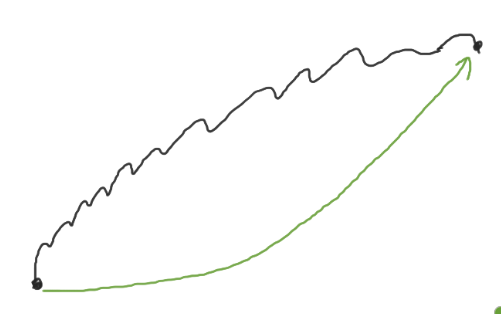
\includegraphics[width=0.25\textwidth]{./images/01Fig5.png}};
          \begin{scope}[x={(image.south east)}, y={(image.north west)}]
          \node at (0.0, 0.0) {};
          \end{scope}
      \end{tikzpicture}
    \end{figure}
    

    Consider a closed system and assume that a heat has been transfered to the system.
    We can move between $S$ and $S + \d S$ by reversible and irreversible paths.
    For the reversible one we have 
    \begin{displaymath}
      \d S  = \frac{\d Q}{T},
    \end{displaymath}
    and for an irreversible proces
    \begin{displaymath}
      \d S \geq \frac{\d Q}{T}.
    \end{displaymath}
    
    \begin{displaymath}
      S(t) = \int_{V(t)} \rho( \vec r , t) s( \vec r, t) \d \vec r,
    \end{displaymath}
    where $s(\vec r, t)$ is entropy per unit volume.
    Entropy balance implies
    \begin{displaymath}
      \dfrac{S}{t} = \frac{\d_e S}{\d t} + \frac{\d_i S}{\d t} 
    \end{displaymath}
    \begin{displaymath}
      \d_e S = \frac{\d Q}{T}.
    \end{displaymath}
    \begin{displaymath}
      \dfrac{S}{t} = \dfrac{}{t} \int_{V(t)} \rho s \d \vec r = \int-\rho \dfrac{s}{t} \d \vec r,
    \end{displaymath}
    \begin{displaymath}
      \dfrac{_e S}{t} = - \int_{\partial V} \frac{ \vec q}{T} \cdot \hat n \d a 
      = - \int_V \nabla \cdot \left( \frac{\vec q}{T} \right) \d \vec r
    \end{displaymath}
    \begin{displaymath}
      \dfrac{_i S}{t} = \int_V \theta \d \vec r,
    \end{displaymath}
    where $\theta$ is the entropy production per unit volume per unit time.
    Thus the \fnte{entropy balance equation} is
    \begin{displaymath}
      \rho \dfrac{s}{t} = - \nabla \cdot \left( \frac{\vec q }{T}  \right) + \theta, \quad \theta \geq 0.
    \end{displaymath}

    For ideal fluid (no internal efects) $\theta = 0$, and the change of entropy
    \begin{displaymath}
      \dfrac{s}{t} = 0.
    \end{displaymath}
\end{document}
